\documentclass[11pt,twocolumn]{article}

% --- Codificación y lenguaje ---
\usepackage[T1]{fontenc}
\usepackage[utf8]{inputenc}
\usepackage[spanish]{babel}

% --- Matemática y fuentes ---
\usepackage{amsfonts, amssymb, amsthm}
\usepackage{amsmath}
\usepackage{derivative}

% --- Gráficos y tablas ---
\usepackage{graphicx}   % ya lo usas
\usepackage{animate}    % paquete para animaciones
\usepackage{caption}        % <-- primero caption
\usepackage{subcaption}     % <-- luego subcaption
\usepackage{booktabs}
\usepackage{ulem} % for \sout
\usepackage{siunitx}

% --- Varios útiles ---
\usepackage[margin=2cm]{geometry}
\usepackage{enumitem}
\usepackage{csquotes}
\usepackage{cuted}          % para elementos a dos columnas (opcional)
\usepackage{stackrel}
\usepackage{float}
\usepackage{placeins}
\usepackage{multirow}
% \usepackage{nameref}      % NO necesario: hyperref ya define \nameref
\usepackage[dvipsnames]{xcolor}
\usepackage{tikz}
\usetikzlibrary{calc}

% --- Bibliografía (BibTeX + apacite) ---
\usepackage[backend=biber,style=apa,language=spanish]{biblatex}
\addbibresource{references.bib} % tu archivo original con @online
\AtBeginBibliography{\raggedright\small}


% --- Hipervínculos (casi al final) ---
\usepackage[
  colorlinks=true,
  linkcolor=black, urlcolor=black, citecolor=black, filecolor=black,
  pdfborder={0 0 0}
]{hyperref}
% --- Colores para hipervínculos (citas en azul) ---
\hypersetup{
  colorlinks=true,
  linkcolor=black,      % refs, índice
  urlcolor=Blue,
  citecolor=Blue   % color del link de la cita
}

% --- Forzar que TODA la cita (no solo el link) salga en color
\makeatletter
\let\orig@cite\cite
\renewcommand{\cite}[1]{\textcolor{Blue}{\orig@cite{#1}}}

% Si en el texto usaste \citeA (cita textual tipo Autor (Año)),
% la convertimos también a formato entre paréntesis y color:
% --- Citas parentéticas y en color, compatible con apacite o biblatex ---
\makeatletter
% ¿Existe \citeA (apacite)? Si no, asumimos biblatex.
\@ifundefined{citeA}{%
  % --------- rama biblatex ---------
  % Si existe \parencite, la coloreamos y mapeamos \cite / \citeA a paréntesis:
  \@ifundefined{parencite}{}{%
    \let\orig@parencite\parencite
    \renewcommand{\parencite}[1]{\textcolor{Blue}{\orig@parencite{#1}}}
    \renewcommand{\cite}[1]{\parencite{#1}}      % \cite -> (Autor, Año)
    \providecommand{\citeA}[1]{\parencite{#1}}   % por si quedó \citeA en el texto
    % (Opcional) forzar \textcite también a parentético:
    % \let\orig@textcite\textcite
    % \renewcommand{\textcite}[1]{\parencite{#1}}
  }%
}{%
  % --------- rama apacite ---------
  \let\orig@cite\cite
  \renewcommand{\cite}[1]{\textcolor{Blue}{\orig@cite{#1}}} % color a (Autor, Año)
  % Hacer que \citeA (Autor (Año)) también salga parentético y en color:
  \let\orig@citeA\citeA
  \renewcommand{\citeA}[1]{\textcolor{Blue}{\orig@cite{#1}}}
}
\makeatother

\begin{document}

% =====================================
% 0. Portada / Encabezado / Abstract.
% =====================================
\begin{tikzpicture}[remember picture,overlay]
  \node[anchor=north east, inner sep=0pt]
    at ($(current page.north east)+(-1.8cm,-1.2cm)$)
    {
\includegraphics[height=2.8cm]{UdeC_logo_azul.png}};
\end{tikzpicture}

\begin{strip}
\begin{center}
\vspace*{-5\baselineskip}
{\Large \textbf{Universidad de Concepción}}\\[-2pt]
\small Facultad de Ciencias Físicas y Matemáticas\\[-2pt]
\small \textit{Física VII Introducción a la Mecánica Cuántica (510322-1)}\\[4pt]

{\Large \bfseries Informe 2: Medición de }\\
[2pt]
{\Large \bfseries la constante de Planck con LEDs}\\
[2pt]
\small Profesor: Paulraj Manidurai\\[-2pt]
\small N. Ulloa C., J. Rosas S.\\[-2pt]
\small Concepción, Chile — 20 de octubre de 2025
\end{center}
\hrule
\begin{center}
\begin{abstract}
Se determinó la constante de Planck empleando diodos emisores de luz (LED) como fuentes cuasimonocromáticas: se registró el voltaje umbral de emisión $\Delta V$ para distintos colores, se representó $\Delta V$ en función de la frecuencia $f$ y se ajustó un modelo lineal $\Delta V = m f + b$. A partir de la pendiente del ajuste, $m \approx h/e$, se estimó $h$ y se evaluó su concordancia con el valor de referencia mediante el error porcentual relativo, obteniendo una constante de Planck experimental de $(5.5\pm0.55)\times10^{-34}\ \mathrm{J\,s}$, con un error relativo al valor visto en la literatura de $16.9\%$.
\end{abstract}
\end{center}

\noindent\rule{\textwidth}{0.4pt}\par\vspace{0.3cm}
\end{strip}

% ===========================
% 1. Objetivos.
% ===========================
\section{Objetivos}
\begin{itemize}
    \item Demostrar la cuantización de la luz a partir de la relación $E=hf$ y la correspondencia $e\,\Delta V = hf$ en LEDs.
    \item Determinar experimentalmente la constante de Planck $h$ a partir de la pendiente de un gráfico $\Delta V$ vs.\ $f$.
    \item Aplicar procedimientos de registro de datos, graficación y análisis de incertidumbres para estimar $h$ y su error porcentual.
\end{itemize}

% ===========================
% 3. Marco teórico.
% ===========================
\section{Fundamento}

\subsection*{Emisión en semiconductores y energía de banda}
En un diodo LED (\textbf{p–n}), cuando se le aplica voltaje para encenderlo, esto hace que las partículas con carga eléctrica (electrones y "huecos") se encuentren en la región de agotamiento del diodo.
Cuando un electrón y un "hueco" se juntan, se combinan. En este proceso, el electrón suelta energía en forma de un fotón.
El color de la luz emitida depende del material con el que esté hecho el LED, porque cada material permite que se emita un color específico, esta energía es la brecha de energía $E_g$.\cite{schubert_leds,streetman_sed,bhattacharya_opto}. En primera aproximación,
\begin{equation*}
    E_\gamma \;\simeq\; h f \;\approx\; E_g,
\end{equation*}
de modo que la longitud de onda central satisface \( \lambda \simeq hc/E_g \) (en el análisis de este informe se usa \(\lambda\) en aire y \(c\) en vacío).

\subsection*{Relación lineal entre el voltaje umbral y la frecuencia}
Cuando el LED comienza a emitir (\textbf{umbral óptico}), la energía eléctrica por carga transferida a través de la unión,
\begin{equation*}
    e\,\Delta V,
\end{equation*}
se reparte en la energía del fotón y en pérdidas no radiativas y/o términos de contacto (caídas serie, reabsorción, eficiencia cuántica interna finita, etc.). Agrupando esas correcciones en un término efectivo \(\Phi\) (de signo tal que incremente el voltaje requerido), resulta el modelo lineal
\begin{align*}
    e\,\Delta V \;&=\; h\,f \;-\; \Phi \\[4pt]
    \Longrightarrow\quad
    \Delta V \;&=\; \underbrace{\frac{h}{e}}_{\text{pendiente } m}\, f \;+\; \underbrace{\Big(-\frac{\Phi}{e}\Big)}_{\text{ordenada } b}\,.
\end{align*}
Bajo estas hipótesis, la pendiente del ajuste \(\Delta V\)–\(f\) estima \(m \approx h/e\) y la ordenada \(b\) cuantifica el sesgo sistemático global del umbral \cite{einstein1905photo,griffiths_em}.

\subsection*{Consecuencias experimentales y supuestos}
El modelo anterior predice: (i) \textbf{linealidad} de \(\Delta V\) con \(f\); (ii) \textbf{pendiente} \(m\) independiente del color/material (si las pérdidas no varían apreciablemente con \(f\)); y (iii) los electrones deben \textbf{superar} el trabajo efectivo \(b\) para ser emitidos. Para sostener la validez de la aproximación se asumió: temperatura aproximadamente constante (variaciones de \(E_g\) con \(T\) despreciables en el rango de trabajo), resistencia serie moderada (caída adicional mínima en el umbral óptico), y selección de \(\lambda\) como longitud de onda pico del fabricante o medida característica, sabiendo que el espectro de emisión tiene un ancho finito \cite{schubert_leds,hecht_optics}.

\subsection*{Magnitudes derivadas y estimación de \(h\)}
A partir del ajuste lineal \(\Delta V = m f + b\), la constante de Planck se obtuvo como
\begin{equation*}
    h \;=\; e\,m,
\end{equation*}
mientras que la comparación con un valor de referencia \(h_{\mathrm{ref}}\) se reportó mediante el error relativo porcentual
\begin{equation*}
    \mathrm{error}_{\%} \;=\; 100\,\frac{\lvert h - h_{\mathrm{ref}}\rvert}{h_{\mathrm{ref}}}\,.
\end{equation*}
La frecuencia se calculó con \( f=c/\lambda \), tomando \(c\) en vacío y \(\lambda\) en aire; cualquier incertidumbre en \(\lambda\) se propaga como \( \delta f \simeq (c/\lambda^2)\,\delta\lambda \) \cite{hecht_optics}.


% ===========================
% 4. Materiales:
% ===========================
\section{Materiales}
\begin{itemize}
    \item Fuente de poder $\sim 2.5\,\mathrm{V}$.
    \item 5 LEDs de colores distintivos.
    \item Resistencia $330\,\Omega$.
    \item Potenciómetro $1\,\mathrm{k}\Omega$ (o resistencia variable).
    \item Protoboard y cables.
    \item Multitester/voltímetro.
\end{itemize}

% ===========================
% 5. Primera experiencia.
% ===========================

\section{Metodología}

\begin{enumerate}
    \item \textbf{Conexión del circuito.} Se realizó el cableado siguiendo el esquema de la Figura~\ref{fig:circuito_de_referencia}. El voltímetro se dispuso en paralelo del LED para medir el voltaje umbral $\Delta V$. Una vista general del montaje se mostró en la Figura~\ref{fig:montaje_general} y el detalle del cableado en protoboard en la Figura~\ref{fig:protoboard_circuito}. Verificar si el LED está en polarización directa.

    \item \textbf{Búsqueda del umbral.} Con el potenciómetro en un valor bajo, se energizó la fuente y se incrementó lentamente la tensión hasta observar el \textbf{primer brillo perceptible y estable} del LED. Se registró el valor de $\Delta V$ indicado por el voltímetro (en paralelo al diodo, cf. Fig.~\ref{fig:circuito_de_referencia}).

    \item \textbf{Barridos de afinamiento.} Se repitieron dos o más barridos alrededor del umbral (incrementando y luego reduciendo la tensión) para afinar la lectura y evaluar la repetibilidad. Se consignaron la media y la dispersión experimental de $\Delta V$.

    \item \textbf{Cambio de color.} Se llevó la perilla del potenciómetro a $0\,\mathrm{V}$, se reemplazó el LED y se repitió el procedimiento anterior para cada color (véanse las Figuras~\ref{fig:circuito_de_referencia} y \ref{fig:protoboard_circuito} para el tendido de conexiones).

    \item \textbf{Tabulación y conversión.} Se tabularon los valores de $\Delta V$ por color y se convirtió la longitud de onda característica $\lambda$ de cada LED en frecuencia mediante $f=c/\lambda$. Estos pares $(f,\Delta V)$ se emplearon en el ajuste lineal $\Delta V = m f + b$ para estimar $m$ y, a partir de $h=e\,m$, la constante de Planck.
\end{enumerate}



\begin{figure}
    \centering
    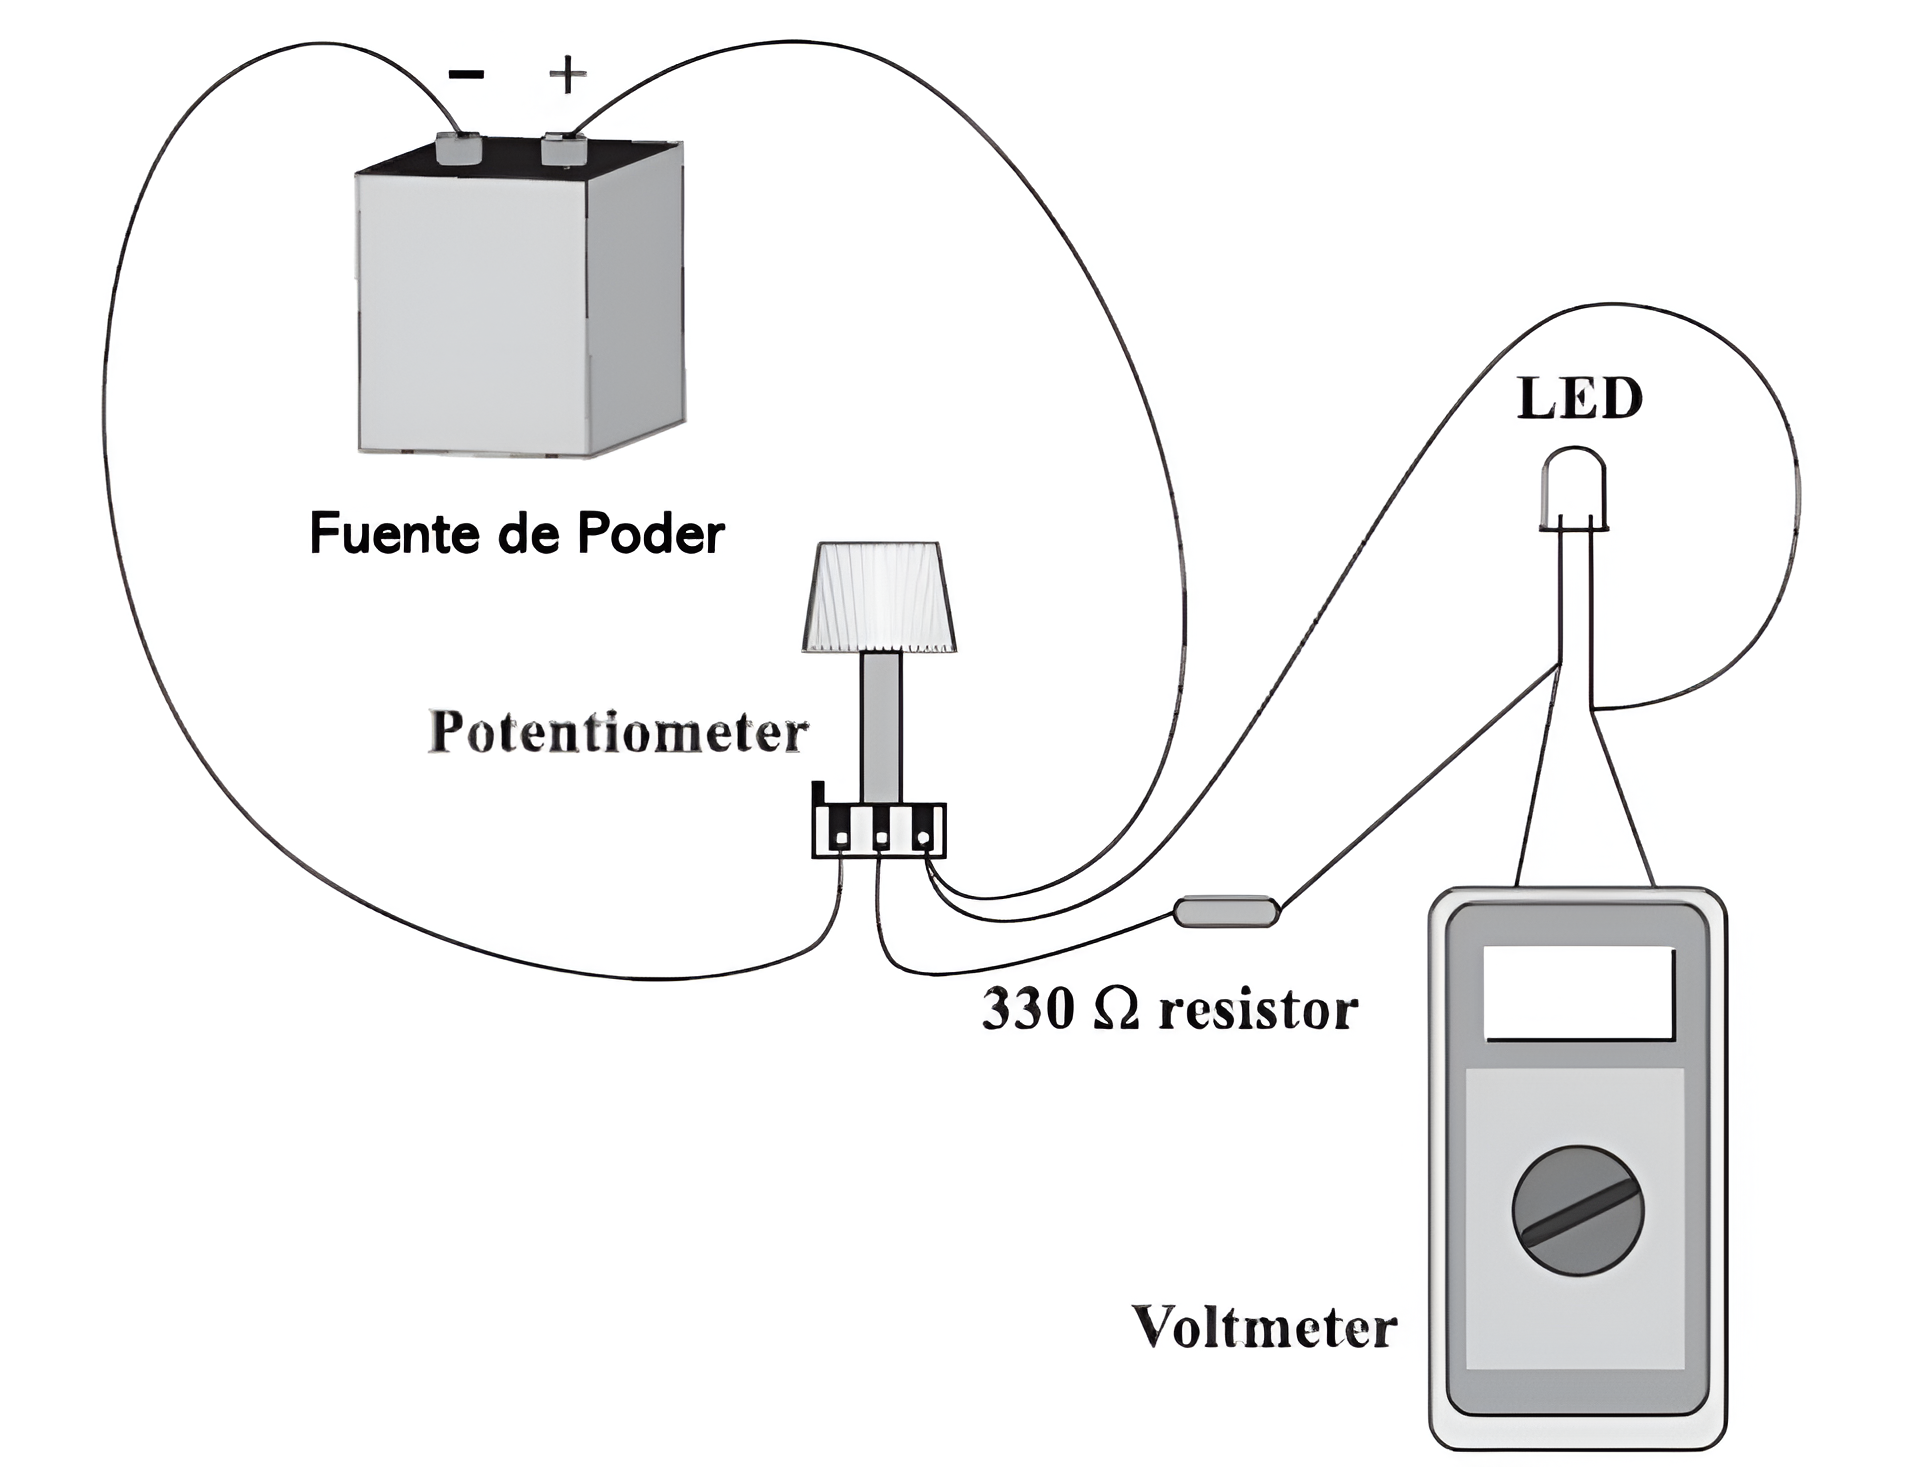
\includegraphics[width=1\linewidth]{figures/circuito_de_referencia.png}
    \caption{Esquema del circuito utilizado para determinar el voltaje umbral del LED. 
    La fuente de poder DC alimenta un potenciómetro en configuración de divisor; el LED se conecta en serie con una resistencia limitadora de $330\,\Omega$ entre el cursor (terminal central) y un extremo del potenciómetro. 
    El voltímetro se conecta en paralelo con el LED para registrar $\Delta V$ al alcanzar el primer brillo perceptible.}
    \label{fig:circuito_de_referencia}
\end{figure}

\begin{figure}
    \centering
    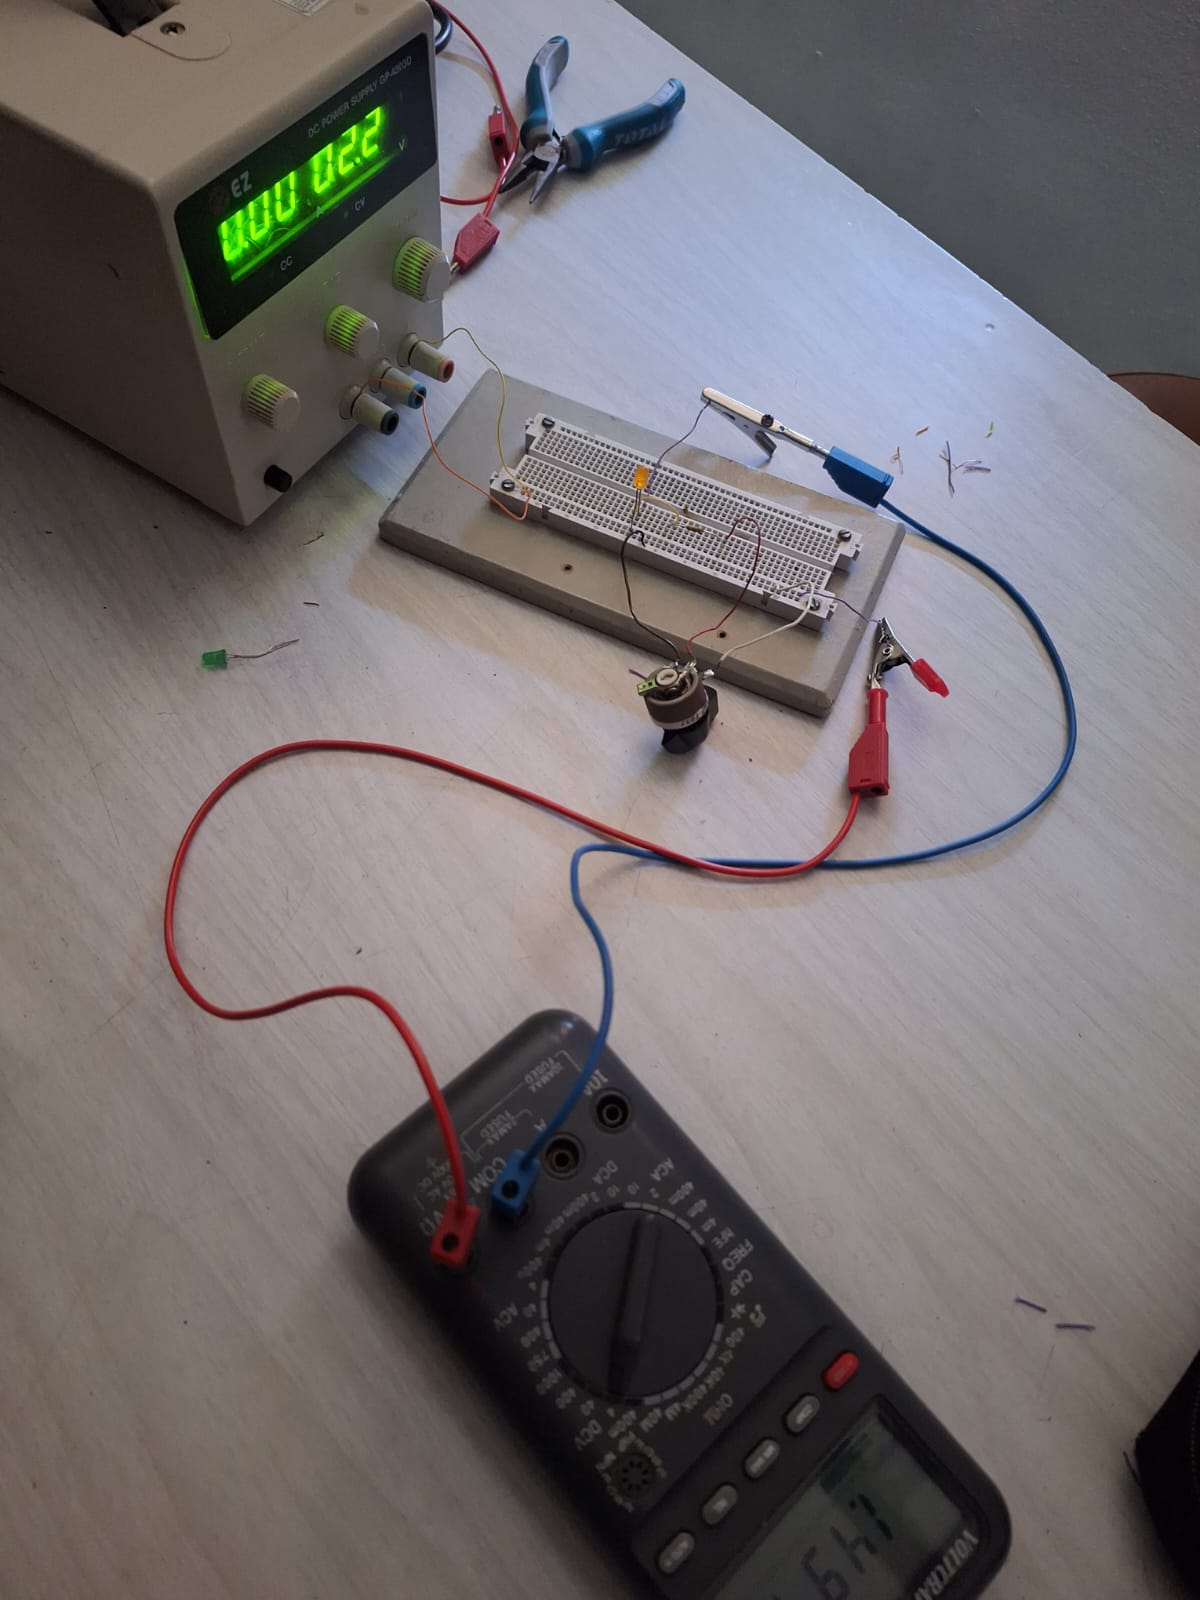
\includegraphics[width=0.8\linewidth]{figures/montaje.jpg}
    \caption{Vista general del montaje experimental: fuente de poder DC, protoboard, potenciómetro y multímetro configurado como voltímetro DC. 
    Durante la medición, el voltímetro se mantuvo en paralelo con el LED mientras se ajustaba el potenciómetro para barrer suavemente la tensión en torno al umbral.}
    \label{fig:montaje_general}
\end{figure}

\begin{figure}
    \centering
    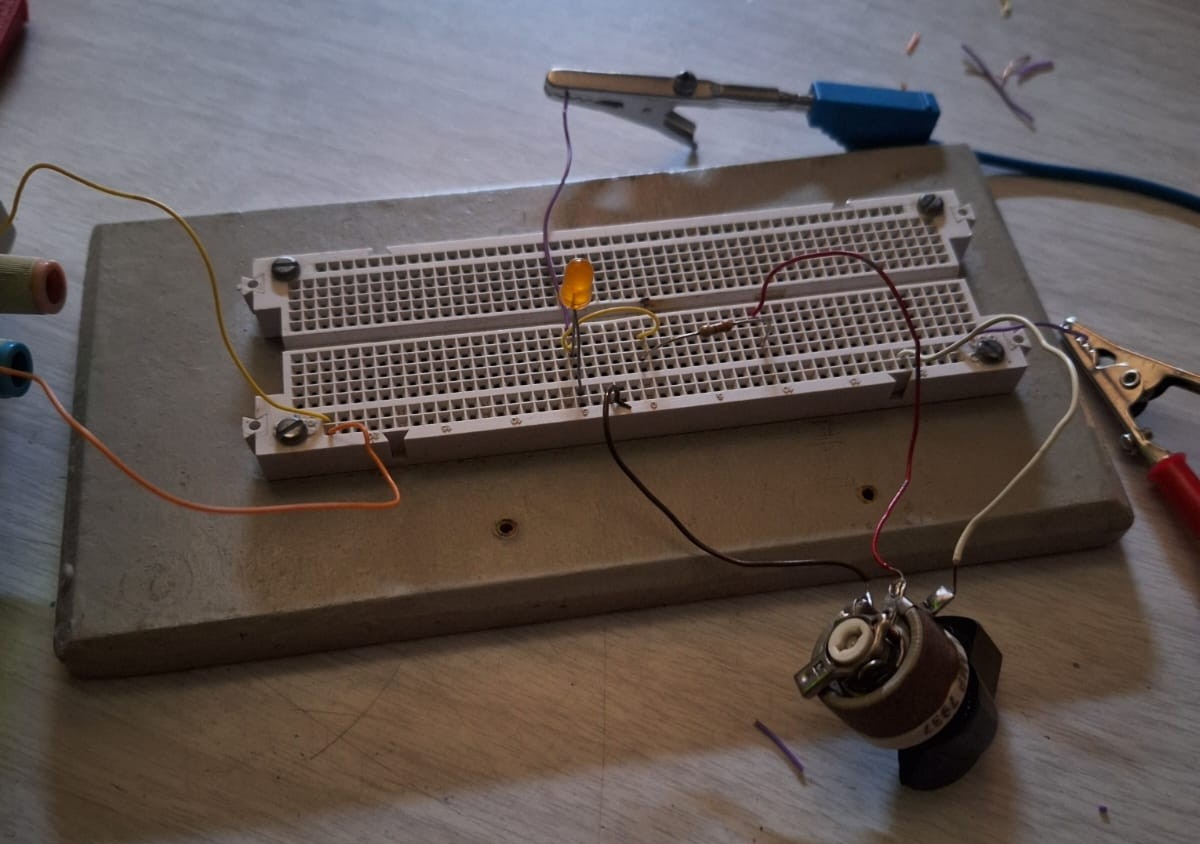
\includegraphics[width=0.9\linewidth]{figures/circuito_montado_en_la_protoboard.jpg}
    \caption{Detalle del cableado en la protoboard. 
    El LED (ánodo–cátodo) está en serie con la resistencia de $330\,\Omega$; el cursor del potenciómetro alimenta el ramal LED–resistencia y los extremos del potenciómetro se conectan a la fuente DC. 
    Esta disposición permitió identificar el umbral como el primer brillo estable del LED y registrar el correspondiente $\Delta V$.}
    \label{fig:protoboard_circuito}
\end{figure}


% ===========================
% 5. Resultados.
% ===========================
\begin{tabular}{cccc}
\hline
\textbf{Color} & $\Delta V$ (V) & $\lambda$ (nm) & $f$ (Hz) \\
\hline
Naranja      & $1.55$        & 600         & $5.00\times10^{14}$ \\
Amarillo     & $1.61$        & 580         & $5.17\times10^{14}$ \\
Verde        & $1.70$        & 532         & $5.64\times10^{14}$ \\
Azul & $2.22$        & 473         & $6.34\times10^{14}$ \\
Rojo & $150$         & 699         & $4.29\times10^{14}$ \\
\hline
\end{tabular}

\vspace{2pt}
\footnotesize{Nota: $\Delta V$ corresponde al voltaje umbral promedio por color; incertidumbre típica en $\Delta V$ $\sim\pm 0.02$ V (lectura/ajuste). La frecuencia $f$ se calcula como $f=c/\lambda$; si $\delta\lambda\!\sim\!\pm1$ nm, entonces $\delta f \approx (c/\lambda^{2})\,\delta\lambda$.}



% ======== Análisis de datos ========
\section{Análisis de datos}

Los pares experimentales $(f,\Delta V)$ se trataron con un modelo lineal
\begin{equation*}
    \Delta V(f) \;=\; m\,f + b \,,
\end{equation*}
en el que $m$ y $b$ representan la pendiente y la ordenada al origen, respectivamente. En el marco del modelo fotoeléctrico para LEDs,
\begin{equation*}
    e\,\Delta V \;=\; h\,f - \Phi 
    \qquad\Longrightarrow\qquad
    m \approx \frac{h}{e}\,,\quad b \approx -\frac{\Phi}{e}\,,
\end{equation*}
por lo que $h$ se obtuvo a partir de $h = e\,m$.

El \textbf{ajuste por mínimos cuadrados ordinarios} (ponderación uniforme) proporcionó estimadores cerrados para $m$ y $b$. Dados $N$ datos $\{(f_i,\Delta V_i)\}_{i=1}^N$,
\begin{align*}
    m &= \frac{\sum_i (f_i-\overline{f})\,\big(\Delta V_i-\overline{\Delta V}\big)}
             {\sum_i (f_i-\overline{f})^2}\,,\\[4pt]
    b &= \overline{\Delta V} - m\,\overline{f}\,,
\end{align*}
donde la barra denota \textbf{promedio muestral}. Asumiendo homocedasticidad\footnote{Se refiere a la igualdad de la varianza (o dispersión) de los errores en un modelo de regresión}, la \textbf{varianza residual} y el término $S_{xx}$ se evaluaron como
\begin{equation*}
    s^2 \;=\; \frac{1}{N-2}\sum_{i=1}^{N}\!\big(\Delta V_i - m f_i - b\big)^2,
    \qquad
    S_{xx} \;=\; \sum_{i=1}^{N} \big(f_i - \overline{f}\big)^2,
\end{equation*}
y la incertidumbre típica de la pendiente se obtuvo de la \textbf{matriz de covarianza} del ajuste:
\begin{align*}
    \delta m \;=\; \sqrt{\mathrm{Var}(m)} \;=\; \sqrt{\frac{s^2}{S_{xx}}}\,,\\[4pt]
    \delta b \;=\; \sqrt{\mathrm{Var}(b)} \;=\; \sqrt{s^2\!\left(\frac{1}{N}+\frac{\overline{f}^{\,2}}{S_{xx}}\right)}.
\end{align*}

La propagación de incertidumbre hacia $h$ fue directa, al ser $e$ exacta en el SI:
\begin{equation*}
    h \;=\; e\,m,
    \qquad
    \delta h \;=\; e\,\delta m,
    \qquad
    \frac{\delta h}{h} \;=\; \frac{\delta m}{m}.
\end{equation*}
La concordancia con el valor de referencia \(h_{\mathrm{ref}}=6.626\times 10^{-34}\,\mathrm{J\,s}\) se cuantificó mediante el error porcentual relativo:
\begin{equation*}
    \mathrm{error}_{\%} \;=\; 100\,\cdot
    \frac{\big|\,h-h_{\mathrm{ref}}\,\big|}{h_{\mathrm{ref}}}\,.    
\end{equation*}

\paragraph*{Presentación y consistencia del ajuste.}
Conforme a lo buscado, se obtuvo
\begin{align*}
    m=(3.4\pm0.35)\times10^{-15}\ \mathrm{V\,Hz^{-1}},\\[4pt]
h=(5.5\pm0.55)\times10^{-34}\ \mathrm{J\,s},\\[4pt]
\mathrm{error}_{\%}=16.9\%.
\end{align*}
En la Fig.~\ref{fig:ajuste_lineal} se aprecia la tendencia lineal de \(\Delta V\) con \(f\) y la obtención de \(m\); los residuos \(r_i=\Delta V_i-(m f_i+b)\) mostrados en la Fig.~\ref{fig:residuos} se distribuyeron alrededor de cero sin patrón sistemático, lo que respaldó la idoneidad del modelo en el rango de trabajo. 
Para transparencia y reproducibilidad, el \textit{script} utilizado en todos los cálculos puede consultarse en \href{https://udeconce-my.sharepoint.com/:u:/g/personal/niulloa2023_udec_cl/IQB2NbhLrADJSIJU2SK48VOWAbXIR97Z7uiEMYvP1ELveDU?e=nXIG5B}{\textcolor{teal}{\texttt{analisis\_planck\_leds.py}}}.


\begin{figure}
    \centering
    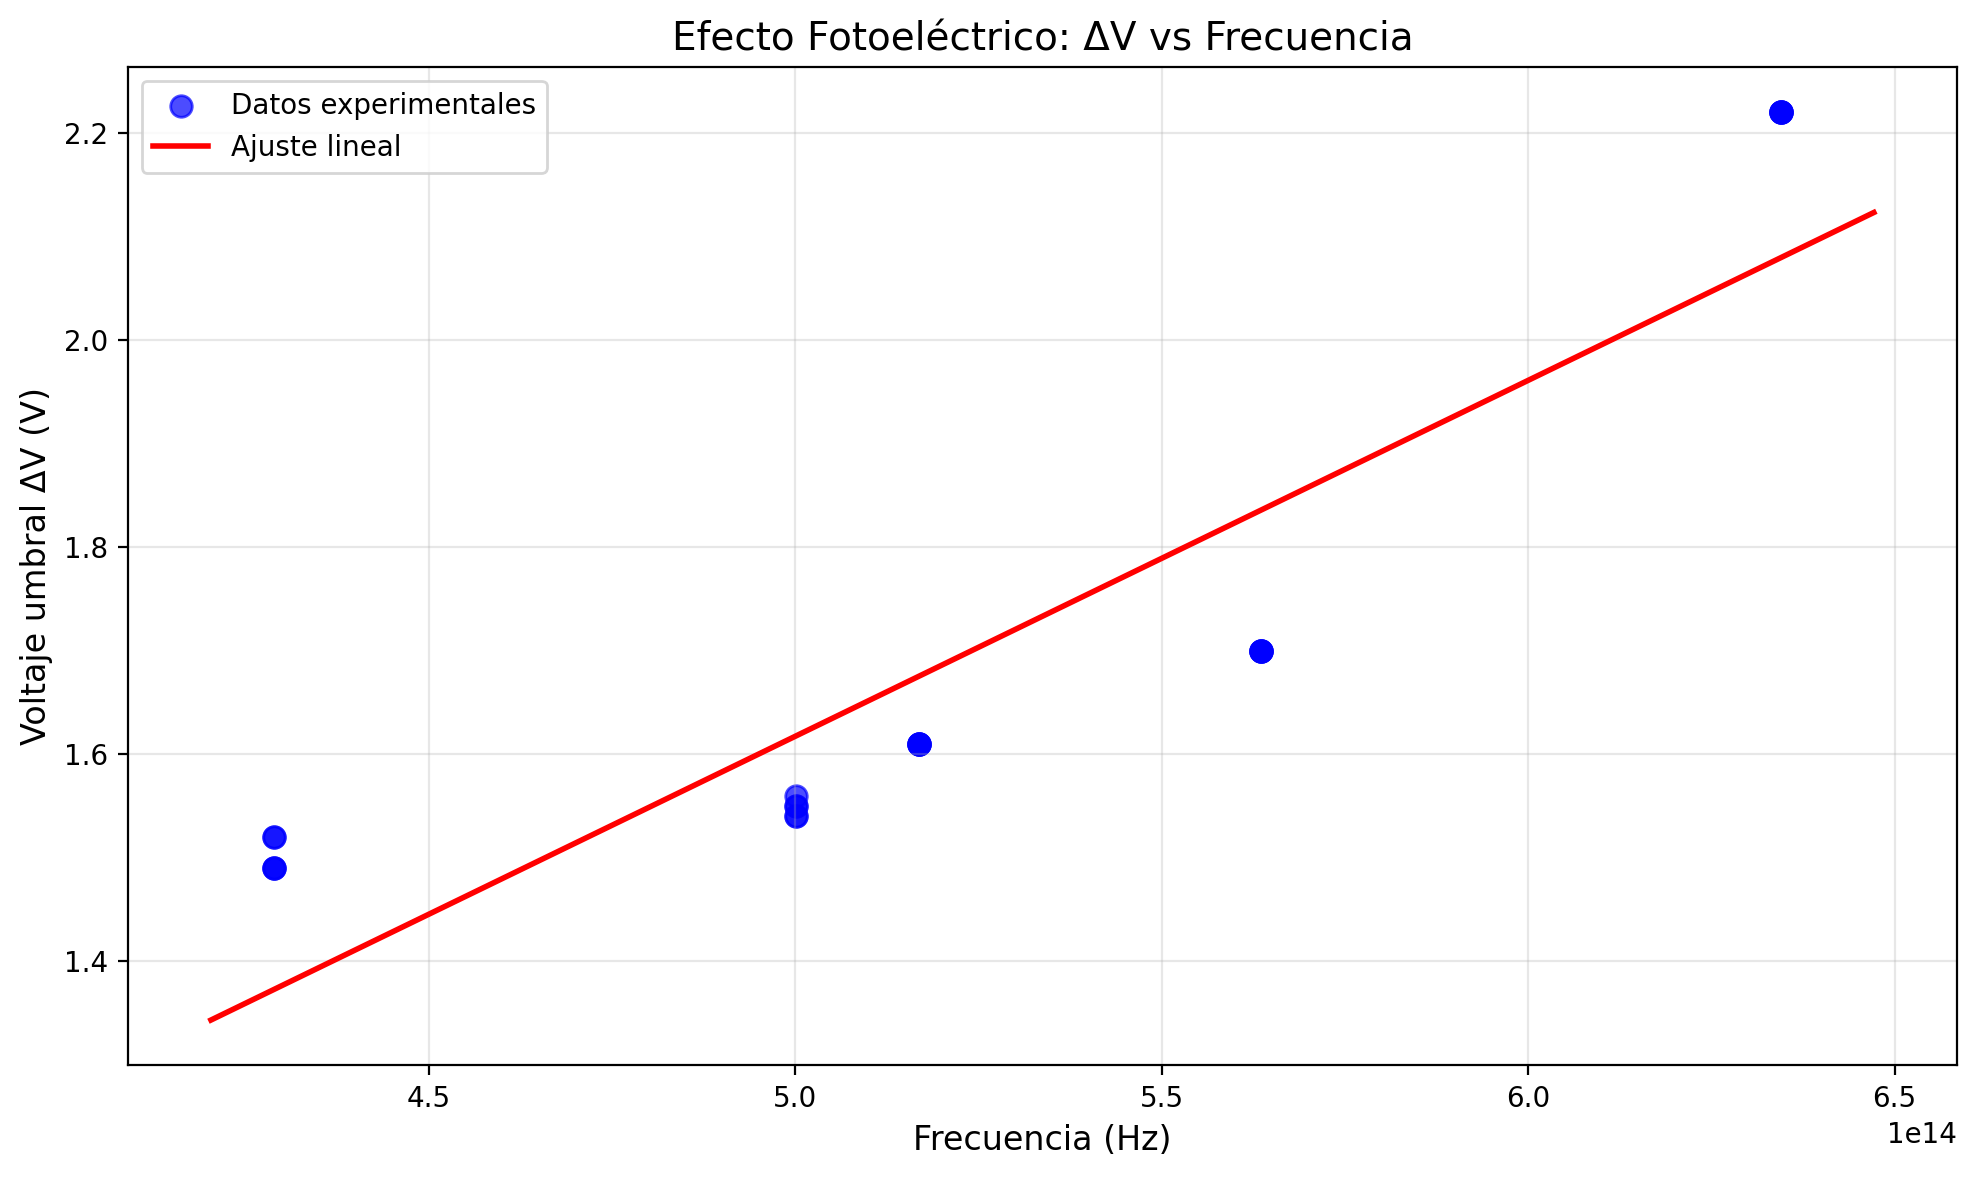
\includegraphics[width=\linewidth]{graphics/ajuste_lineal_efecto_fotoelectrico.png}
    \caption{Ajuste lineal de $\Delta V$ en función de la frecuencia $f$. 
    Los puntos representan los promedios experimentales por color de LED y la línea roja indica la recta de mínimos cuadrados. 
    La pendiente $m$ se relacionó con la constante de Planck mediante $h=e\,m$, mientras que la ordenada $b$ aproxima $-\Phi/e$ (trabajo de extracción efectivo). 
    Las barras de error en $f$ son despreciables frente a las de $\Delta V$ en este montaje.}
    \label{fig:ajuste_lineal}
\end{figure}

\begin{figure}
    \centering
    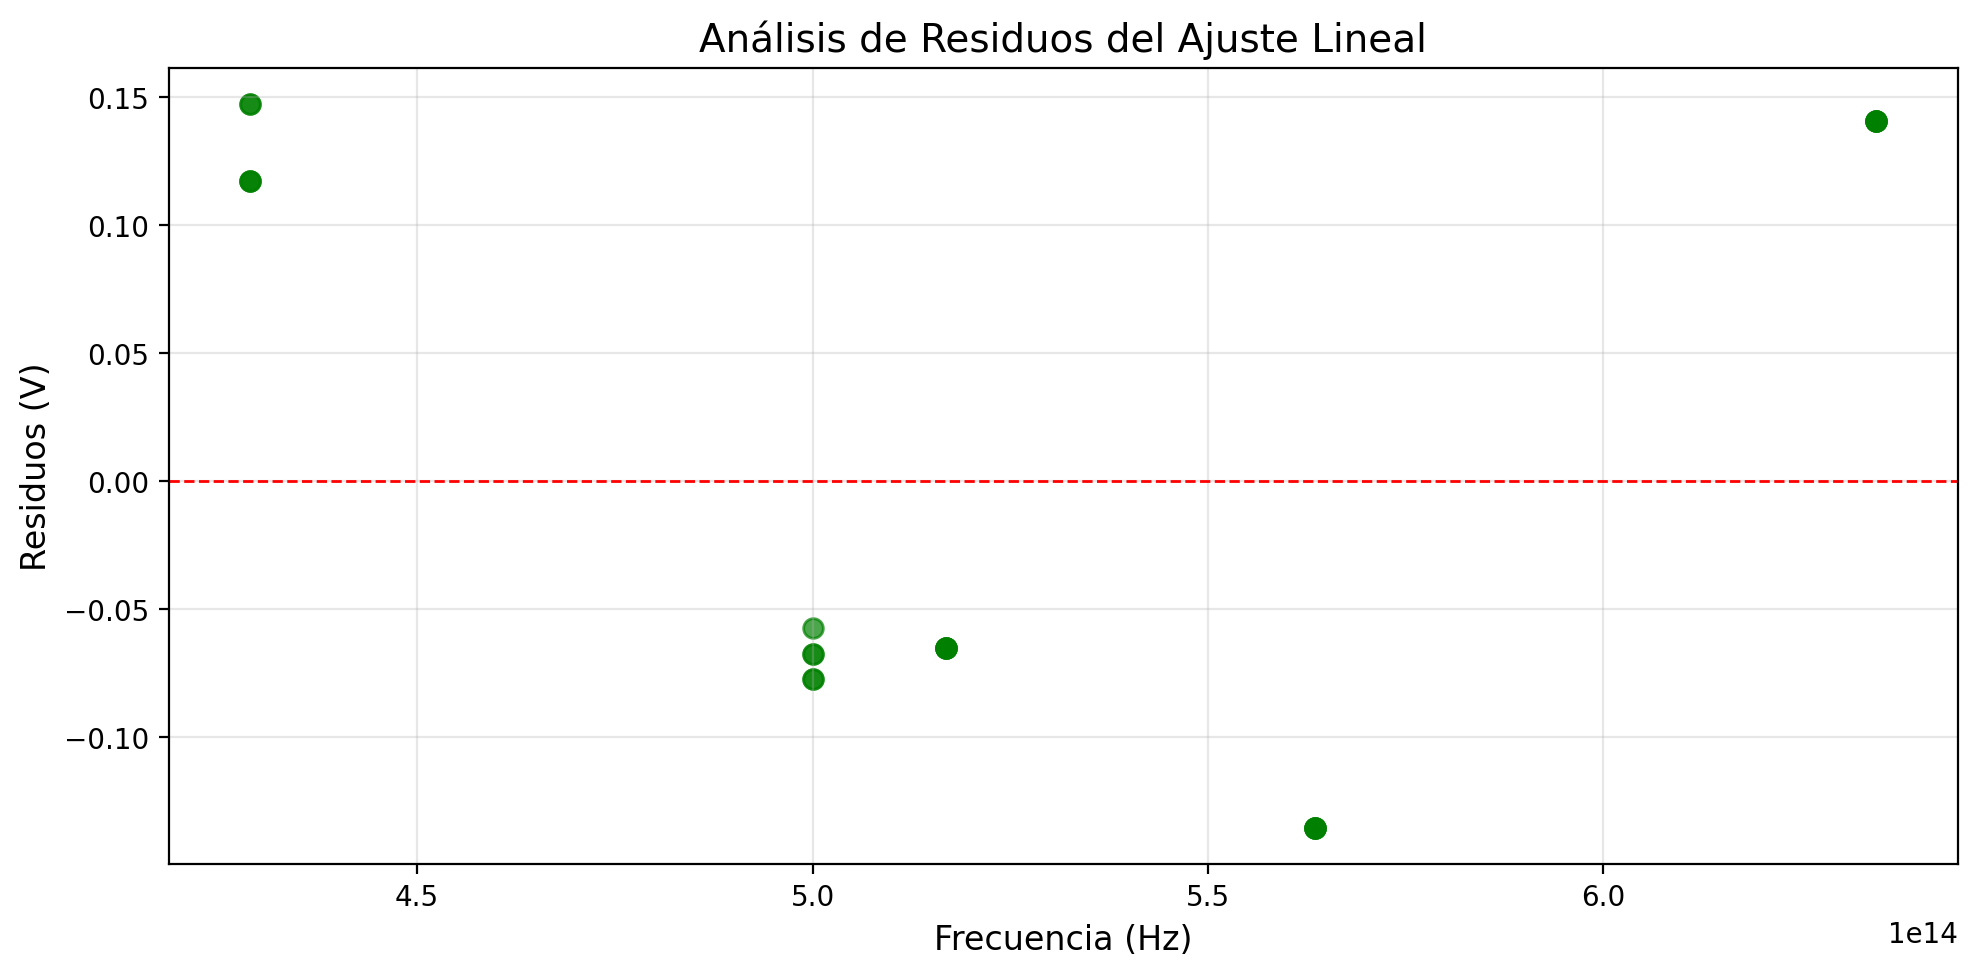
\includegraphics[width=\linewidth]{graphics/residuos_ajuste.png}
    \caption{Residuos del ajuste, $r_i=\Delta V_i-(m f_i+b)$, en función de $f$. 
    La línea discontinua marca $r_i=0$. 
    La dispersión aproximadamente simétrica y la ausencia de patrón monotónico sugieren homocedasticidad y validez del modelo lineal en primera aproximación; los pocos desvíos más grandes identifican las condiciones donde la lectura del umbral pudo ser menos precisa.}
    \label{fig:residuos}
\end{figure}

\section{Discusión de errores}
Se identificaron fuentes de incertidumbre \textit{aleatoria} y \textit{sistemática}. Entre las aleatorias, dominaron: (i) la lectura del \emph{primer brillo perceptible} del LED, (ii) la resolución del voltímetro y la estabilidad de la fuente, y (iii) la dispersión en \(\lambda\) propia del LED (ancho espectral), que induce \(\delta f \simeq (c/\lambda^{2})\,\delta\lambda\). Entre las sistemáticas, destacaron: (i) caídas de voltaje perdidas en el contacto, (ii) recombinación no radiativa y reabsorción que elevan el umbral óptico (término efectivo \(b\simeq -\Phi/e\)), y (iii) la deriva térmica de \(E_g\) con la temperatura. Estas contribuciones se reflejaron en el intercepto \(b\) y en la varianza de la pendiente \(m\).

El ajuste por mínimos cuadrados ordinarios entregó \(m\) y \(b\) junto con sus incertidumbres a partir de la matriz de covarianza: \(\delta m=\sqrt{\mathrm{Var}(m)}\). La propagación hacia \(h\) fue directa (con \(e\) exacta): \(h=e\,m\), \(\delta h=e\,\delta m\) y \(\delta h/h=\delta m/m\). La consistencia del modelo se evaluó inspeccionando los residuos \(r_i=\Delta V_i-(m f_i+b)\): ausencia de tendencias sistemáticas y dispersión aproximadamente con varianza constante respaldaron la idoneidad de la relación lineal en el rango de trabajo. Como buenas prácticas adicionales, se recomienda: (i) ponderar el ajuste si las incertidumbres de \(\Delta V\) difieren entre colores; (ii) aumentar el número de mediciones y la cobertura en \(f\); (iii) objetivar el criterio de umbral con un fotodiodo; y (iv) estimar \(\lambda\) con espectrómetro para reducir \(\delta f\).

\section{Conclusiones}
El análisis de \(\Delta V\) frente a \(f\) exhibió la dependencia lineal esperada y permitió estimar la constante de Planck a partir de la pendiente del ajuste. Se obtuvo
\begin{align*}
    m=(3.4\pm0.35)\times10^{-15}\ \mathrm{V\,Hz^{-1}},\\[4pt]
h=(5.5\pm0.55)\times10^{-34}\ \mathrm{J\,s},\\[4pt]
\mathrm{error}_{\%}=16.9\%.
\end{align*}
valores que resultaron razonablemente coherentes con la referencia dentro de las incertidumbres reportadas. La inspección de residuos apoyó la adecuación del modelo y sugiere que las discrepancias restantes se deben principalmente a sesgos instrumentales y de umbral, mitigables con las mejoras metodológicas indicadas.

\printbibliography

\end{document}
